% note.tex — φ^3+φ^4 理論の有限温度の一次相転移と重力波
% コンパイル: lualatex note.tex（目次と参照の解決のため2〜3回）
\documentclass[a4paper,10pt]{ltjsarticle}
\usepackage[margin=20mm]{geometry}
\usepackage[haranoaji,deluxe]{luatexja-preset}
\ltjsetparameter{jacharrange={-3}}
\usepackage{amsmath,amssymb}
\usepackage{booktabs,tabularx,array}
\usepackage[table]{xcolor}
\usepackage[font=small,labelfont=bf]{caption}
\usepackage{graphicx}
\usepackage{placeins}
\usepackage{xurl}
\usepackage{hyperref}
\hypersetup{colorlinks=true,linkcolor=blue!50!black,citecolor=green!40!black,urlcolor=blue!60!black,
  pdftitle={phi^3+phi^4 theory: first-order phase transition at finite temperature and gravitational waves},pdfauthor={}}

\renewcommand{\jsParagraphMark}{\textcolor{black!65}{\rule[-0.02\zw]{0.62\zw}{0.62\zw}}\hspace{0.35\zw}}
\newcommand{\dd}{\mathrm{d}}

\title{$\phi^3+\phi^4$ 理論の有限温度の一次相転移と重力波}
\author{}
\date{2026年10月12日}

\begin{document}
\maketitle

\begin{abstract}
零温度の $\phi^3+\phi^4$ 理論のノート~\cite{phi34note} に続き、有限温度の一次相転移を調べる。零温度のノートで求めた3次元の bounce の作用 $S_3(\alpha)$ を使い、相転移の温度、強さ、速さと、それが作る重力波を求めることが目的である。温度の模型は二つ使う。一つは、Dine ら~\cite{dine92} の高温展開の一般形 $D(T^2-T_0^2)\phi^2-ET\phi^3+\lambda_T\phi^4/4$ で、もう一つは、場 $\phi$ 自身の熱ループだけで閉じた本模型の温度ポテンシャルである。手計算では、一般形が零温度の模型と $\alpha(T)=(\lambda_TD/E^2)(1-T_0^2/T^2)$ で対応することを示し、臨界温度、$S_3/T=(E/36)(2\alpha/\lambda_T)^{3/2}S_3(\alpha)$、核生成の条件、$\beta/H$ の閉じた式を導いた。手順 (1) では、今の質量を入れた SM 的な係数で、臨界温度が閉じた式と数値の極小で全桁一致し、核生成温度は $T_c$ の $0.017$~GeV 下、$S_3/T=148.8$、$\beta/H=2.5\times10^6$、$\phi_n/T_n=0.17$ の弱い一次相転移になった。$S_3/T$ は Dine らの近似式と $0.9\%$ で、$\beta/H$ の閉じた式は数値微分と相対 $4\times10^{-9}$ で一致した。手順 (2) では、相転移の強さを Caprini ら~\cite{caprini20} の $\alpha_\theta=4\Delta\theta/(3w_+)$ で測り、手計算で $\Delta\theta=DT_0^2\phi_n^2/2$、すなわち $\alpha_\theta=(15D/\pi^2g_*)(T_0/T_n)^2(\phi_n/T_n)^2$ を導いた。$T_0$ を含む項のほかは $T^4$ に比例してトレースを持たないので、強さは $\phi_n/T_n$ と過冷却の度合い $T_0/T_n$ だけで決まる。$E$ と $\lambda_T$ を変えた走査では、$\phi_n/T_n$ は最大 $7.2$、$\alpha_\theta$ は最大 $0.071$、$\beta/H$ は最小 $7.5\times10^2$ だった。手順 (3) では、音波と乱流による重力波を原論文の式で求め、LISA の要求感度と比べた。最も強い点（$\alpha_\theta=0.071$、$\beta/H=974$、壁の速さ $0.95$）でも、ピークは $f=20$~mHz で $h^2\Omega_{\mathrm{gw}}=2.0\times10^{-15}$、SNR は $0.014$ で、検出の目安の SNR $=10$ に届かない。SNR $=10$ には、この強さのままなら $\beta/H\lesssim134$、この速さのままなら $\alpha_\theta\gtrsim2$ が要る。導出はすべて付録に省略なく載せる。
\end{abstract}

\tableofcontents

\section{目的と問い}\label{sec:intro}

本ノートの問いは二つである。\textbf{第一に、零温度のノートで検算した3次元の bounce の作用を使うと、有限温度の一次相転移の温度、強さ、速さと、それが作る重力波はどう決まるか。第二に、$\phi^3+\phi^4$ 理論そのものの熱的な歴史では、高温の相からどちらの真空に移るか。そして、それは零温度のノートの真空の安定性の限界をどう変えるか。}

第一の問いを立てる理由は、零温度のノートの手順 (9) で、$d=3$ の作用 $S_3(\alpha)$ を Dine ら~\cite{dine92} の近似式と $0.8\%$ 以内で一致させてあるからである。電弱相転移の高温展開のポテンシャル $D(T^2-T_0^2)\phi^2-ET\phi^3+\lambda_T\phi^4/4$ は、温度に依存する係数を持つ $\phi^3+\phi^4$ のポテンシャルそのものなので、$S_3(\alpha)$ をそのまま使える。第二の問いを立てる理由は、零温度のノートで $\alpha<1$ の $\phi=0$ を準安定な真空として扱ったが、宇宙が高温から冷えるとき、そもそも $\phi=0$ に落ち着くかは自明でないからである。

求める量は四つである。(i) 一般形の臨界温度と、零温度の $\alpha$ との対応。(ii) 核生成温度 $T_n$、相転移の強さ $\alpha_{\mathrm{PT}}$、速さ $\beta/H$。(iii) 音波と乱流による重力波のスペクトルと、LISA の感度との比較。(iv) 場 $\phi$ 自身の熱ループによる温度ポテンシャルでの、相の移り変わりと $(\kappa_3,\kappa_4)$ の熱的な安定性。

本ノートの構成は次の通りである。第~\ref{sec:setup} 節で模型と前提を定める。第~\ref{sec:results} 節で手計算の結果を述べる。第~\ref{sec:plan} 節で検算と計算の計画を定める。第~\ref{sec:dine} 節で一般形の相転移を扱う（現在は手順 (3) まで）。第~\ref{sec:discussion} 節で未決の点と今後の手順をまとめる。導出は\ref{app:map}〜\ref{app:gw} にある。

\section{設定}\label{sec:setup}

零温度のノート~\cite{phi34note} の模型は、ポテンシャル $V=\frac12m^2\phi^2+\frac g{3!}\phi^3+\frac\lambda{4!}\phi^4$ を持つ実スカラー1つで、その形は $\alpha\equiv3\lambda m^2/g^2$ で決まる。有限温度では、高温展開の一般形
\begin{equation}
V(\phi,T)=D\,(T^2-T_0^2)\,\phi^2-ET\phi^3+\frac{\lambda_T}{4}\phi^4
\label{eq:VT}
\end{equation}
を使う~\cite{dine92}。$D$、$E$、$T_0$、$\lambda_T$ は温度にほとんどよらない係数で、SM ではゲージ粒子とトップクォークの熱ループから決まる（\ref{app:map}）。場 $\phi$ 自身の熱ループによる温度ポテンシャルは、後の手順で導く。

\paragraph{前提。}本ノートは次の前提に立つ。
\begin{enumerate}
\item $\hbar=c=k_B=1$ とし、エネルギーと温度の単位は GeV とする。
\item 宇宙は放射優勢で、有効自由度は $g_*=106.75$、ハッブル率は $H=1.66\sqrt{g_*}\,T^2/M_{\mathrm{Pl}}$（$M_{\mathrm{Pl}}=1.22091\times10^{19}$~GeV）とする。
\item 有限温度の崩壊率は $\Gamma(T)=T^4\bigl(S_3/(2\pi T)\bigr)^{3/2}e^{-S_3/T}$ とし~\cite{linde83}、核生成温度 $T_n$ を $\Gamma(T_n)=H(T_n)^4$ で定める。前因子は見積もりで、その不定性は $T_n$ の条件の対数にしか効かない。
\item 一般形の係数は1ループの高温展開の値で、$\lambda_T$ の温度依存（対数）は $T_c$ での値で代表させる。Dine らによれば、$\lambda_T$ の $T_1$、$T_c$、$T_0$ での値の差は小さい。
\item SM 的な係数には、$m_W=80.37$、$m_Z=91.19$、$m_t=172.6$、$m_h=125.25$、$v=246.22$（いずれも GeV）を使う。
\item 相転移の強さと速さは $T_n$ で評価する。式~\eqref{eq:VT} は、$\phi$ によらない放射の自由エネルギー $-\pi^2g_*T^4/90$ を除いた部分とし（$V(0,T)=0$）、対称相のエンタルピー密度は放射のもの $w_+=\frac43\rho_{\mathrm{rad}}$（$\rho_{\mathrm{rad}}=\pi^2g_*T^4/30$）とする。
\item 重力波は、泡の壁が一定の速さ $v_w$ で広がり（暴走しない）、放出されたエネルギーが流体の運動に移る場合の、音波と乱流から求める。$v_w$ は模型からは決めず、$0.95$（デトネーション）と $0.44$（デフラグレーション）の二つを使う。発生時の温度 $T_*$ は $T_n$ とし（再加熱は無視）、その後の宇宙は放射優勢で断熱的に膨張するとする。今日のハッブル定数は $h=0.678$、CMB の温度は $2.725$~K とする。
\item LISA は、4年の観測で稼働率 $75\%$（$T_{\mathrm{obs}}=9.46\times10^7$~s）とし、検出の目安を SNR $=10$ とする。
\end{enumerate}
本文で使う記号を表~\ref{tab:notation} にまとめる。

\begin{table}[tbp]
\centering\small
\caption{本ノートで使う記号。}
\label{tab:notation}
\begin{tabularx}{\linewidth}{>{\raggedright\arraybackslash}p{3.6cm}X}
\toprule
\textbf{記号} & \textbf{意味} \\
\midrule
$D,\ E,\ T_0,\ \lambda_T$ & 一般形 \eqref{eq:VT} の係数 \\
$M^2(T)$ & $\phi=0$ のまわりの有効質量の2乗 $2D(T^2-T_0^2)$ \\
$\alpha(T)$ & 零温度のノートの $\alpha$ を温度の関数として読んだもの（式~\eqref{eq:alphaT}） \\
$R$ & $\lambda_TD/E^2$。$\alpha(T)=R(1-T_0^2/T^2)$ \\
$T_1,\ T_c,\ T_0$ & 二つ目の極小が現れる温度、二つの極小が縮退する温度、$\phi=0$ が不安定になる温度 \\
$S_3(\alpha)$ & 零温度のノートの3次元の bounce の作用（$S_3=S_3(\alpha)\,m^3/g^2$） \\
$W(\alpha)$ & $\dd S_3(\alpha)/\dd\alpha$ \\
$\Gamma,\ H,\ g_*,\ M_{\mathrm{Pl}}$ & 単位体積・単位時間あたりの核生成率、ハッブル率、有効自由度、Planck 質量 \\
$T_n$ & 核生成温度（$\Gamma=H^4$） \\
$\beta/H$ & 相転移の速さ $T\,\dd(S_3/T)/\dd T$（$T=T_n$） \\
$\phi_-,\ \phi_c,\ \phi_n$ & 二つ目の極小の場の値と、その $T_c$、$T_n$ での値 \\
$e,\ p,\ w,\ \theta$ & エネルギー密度、圧力、エンタルピー密度 $e+p$、トレースの $1/4$ にあたる $(e-3p)/4$ \\
$\rho_{\mathrm{rad}}$ & 放射のエネルギー密度 $\pi^2g_*T^4/30$ \\
$\Delta V,\ \Delta\theta,\ \Delta e$ & 対称相（$\phi=0$、添字 $+$）から破れた相（$\phi_-$、添字 $-$）を引いた差 \\
$\alpha_\theta,\ \alpha_e$ & 相転移の強さ $4\Delta\theta/(3w_+)$、$4\Delta e/(3w_+)$（$T=T_n$） \\
$v_w,\ c_s$ & 泡の壁の速さ、音速 $1/\sqrt3$ \\
$\kappa,\ K,\ \bar U_f$ & 流体の運動への効率、流体の運動エネルギーの割合 $\kappa\alpha_\theta/(1+\alpha_\theta)$、流体の速さの2乗平均の平方根（$K=\frac43\bar U_f^2$） \\
$T_*,\ H_*,\ R_*,\ \tau_{\mathrm{sh}}$ & 重力波が生じるときの温度とハッブル率、泡の平均間隔、衝撃波ができるまでの時間 \\
$h^2\Omega_{\mathrm{gw}}(f)$ & 今日の重力波のエネルギー密度の $\ln f$ あたりの値を臨界密度で割ったもの（$h=H_0/(100$~km/s/Mpc$)$） \\
$F_{\mathrm{gw},0},\ H_{*,0},\ f_p$ & 今日までの薄まりの因子、$H_*$ を今日の周波数に直したもの、音波のスペクトルのピークの周波数 \\
$S_h,\ h^2\Omega_{\mathrm{sens}}$ & LISA の歪みの感度（片側のスペクトル密度）と、それを $h^2\Omega$ に直したもの \\
SNR、PLS & 信号対雑音比と、べき乗のスペクトルに対する感度（power-law sensitivity） \\
\bottomrule
\end{tabularx}
\end{table}

\section{結果}\label{sec:results}

\paragraph{零温度の模型との対応。}式~\eqref{eq:VT} は、$m^2=M^2(T)\equiv2D(T^2-T_0^2)$、$g=-6ET$、$\lambda=6\lambda_T$ とした零温度の模型のポテンシャルである。したがって
\begin{equation}
\alpha(T)=\frac{\lambda_TM^2}{2E^2T^2}=R\Bigl(1-\frac{T_0^2}{T^2}\Bigr),\qquad R\equiv\frac{\lambda_TD}{E^2}
\label{eq:alphaT}
\end{equation}
で、これは Dine らの $\alpha$ と同じである（\ref{app:map}）。零温度のノートの真空の構造（$\alpha>9/8$ で極小は一つ、$\alpha=1$ で縮退、$\alpha<1$ で $\phi=0$ が準安定）が、そのまま温度の関数として読める。高温（$\alpha>9/8$）から冷えると、$\alpha=9/8$ で二つ目の極小が現れ、$\alpha=1$ で二つの極小が縮退し、$\alpha=0$ で $\phi=0$ が不安定になる。その温度と場の値は
\begin{equation}
T_1^2=\frac{T_0^2}{1-9E^2/(8\lambda_TD)},\quad\phi_1=\frac{3ET_1}{2\lambda_T};\qquad
T_c^2=\frac{T_0^2}{1-E^2/(\lambda_TD)},\quad\phi_c=\frac{2ET_c}{\lambda_T};\qquad
\phi_0=\frac{3ET_0}{\lambda_T}
\label{eq:crit}
\end{equation}
で、Dine らの式 (12)〜(16) を再現する（\ref{app:map}）。

\paragraph{3次元の作用。}零温度のノートの $S_3=(m^3/g^2)S_3(\alpha)$ に上の対応を入れると
\begin{equation}
\frac{S_3}{T}=\frac{M^3}{36E^2T^3}\,S_3(\alpha)=\frac{E}{36}\Bigl(\frac{2\alpha}{\lambda_T}\Bigr)^{3/2}S_3(\alpha)
\label{eq:S3T}
\end{equation}
となる（\ref{app:map}）。温度は $\alpha(T)$ を通してだけ入る。Dine らの近似式 $S_3/T=4.85\,M^3/(E^2T^3)\,f(\alpha)$ は、$S_3(\alpha)=36\times4.85\,f(\alpha)$ にあたる。

\paragraph{核生成と相転移の速さ。}$\Gamma=H^4$ は
\begin{equation}
\frac{S_3}{T}-\frac32\ln\frac{S_3}{2\pi T}=4\ln\frac{M_{\mathrm{Pl}}}{1.66\sqrt{g_*}\,T}
\label{eq:nucl}
\end{equation}
と書ける（\ref{app:nucl}）。右辺は $T\approx160$~GeV で $144$ で、よく使われる $S_3/T\approx140$ の目安にあたる。相転移の速さは、$\lambda_T$ を一定とすると
\begin{equation}
\frac\beta H=T\frac{\dd}{\dd T}\frac{S_3}{T}=\frac{S_3}{T}\Bigl[\frac{3}{2\alpha}+\frac{W(\alpha)}{S_3(\alpha)}\Bigr]\cdot2(R-\alpha)
\label{eq:betaH}
\end{equation}
である（\ref{app:nucl}）。$W=\dd S_3(\alpha)/\dd\alpha$ は零温度のノートの手順 (9) で求めてある。

\paragraph{相転移の強さ。}Caprini ら~\cite{caprini20} の式 (12) に従い、相転移の強さを $\alpha_\theta=4\Delta\theta(T_n)/(3w_+(T_n))$ で測る。$\theta=(e-3p)/4$ はエネルギー運動量テンソルのトレースの $1/4$ で、bag 模型では $\Delta\theta$ が bag 定数そのものになる。ポテンシャルの差を圧力の差 $p_+-p_-=-(V(0,T)-V(\phi_-,T))$ と読み、極小の条件を使うと
\begin{equation}
\Delta\theta=\frac12DT_0^2\phi_-^2,\qquad
\alpha_\theta=\frac{\Delta\theta}{\rho_{\mathrm{rad}}}=\frac{15D}{\pi^2g_*}\Bigl(\frac{T_0}{T_n}\Bigr)^2\Bigl(\frac{\phi_n}{T_n}\Bigr)^2
\label{eq:alphatheta}
\end{equation}
となる（\ref{app:strength}）。式~\eqref{eq:VT} のうち $T_0$ を含む項のほかは $(\phi,T)$ について4次の斉次式で、$T^4$ に比例する自由エネルギーは放射と同じくトレースを持たない。そのため $\Delta\theta$ は $T_0$ という尺度だけから生じる。強さは $\phi_n/T_n$ と過冷却の度合い $T_0/T_n$ だけで決まり、$E$ と $\lambda_T$ には $\phi_n/T_n$ と $T_n$ を通してだけよる。$\alpha>0$ で核生成が起こるかぎり $T_n>T_0$ なので、$\alpha_\theta<(15D/\pi^2g_*)(\phi_n/T_n)^2$ が上限になる。$T_c$ では $4\Delta\theta$ は潜熱 $L=2DT_0^2\phi_c^2$ に等しい。Caprini らの式 (13) の、エネルギーの差による強さ $\alpha_e=4\Delta e(T_n)/(3w_+(T_n))$ は
\begin{equation}
\Delta e=4\Delta\theta-3\Delta V,\qquad \Delta V=V(0,T)-V(\phi_-,T)=\frac{\phi_-^2}{4}\bigl(ET\phi_--M^2\bigr)
\label{eq:alphae}
\end{equation}
から求まる（\ref{app:strength}）。

\paragraph{重力波の式。}泡の壁が広がると、放出されたエネルギーの一部が流体の運動になり、その音波と乱流が重力波を出す。流体の運動エネルギーの割合は $K=\kappa\,\alpha_\theta/(1+\alpha_\theta)$ で~\cite{caprini20}、効率 $\kappa(\alpha_\theta,v_w)$ には Espinosa ら~\cite{espinosa10} の近似式を使う。指数関数的に増える核生成率のもとでは、泡の平均間隔は $H_*R_*=(8\pi)^{1/3}\max(v_w,c_s)/(\beta/H)$ である（\ref{app:gw}）。音波による今日のスペクトルには、Hindmarsh ら~\cite{hhrw17} の数値シミュレーションの式（正誤表で直したもの）を使う。
\begin{equation}
h^2\Omega_{\mathrm{sw}}(f)=h^2\cdot3\times0.687\,F_{\mathrm{gw},0}\,K^2\,(H_*R_*)\,\tilde\Omega_{\mathrm{gw}}\,C\Bigl(\frac f{f_p}\Bigr)\min\bigl(1,H_*\tau_{\mathrm{sh}}\bigr),\qquad
C(s)=s^3\Bigl(\frac7{4+3s^2}\Bigr)^{7/2}
\label{eq:Osw}
\end{equation}
ここで $\tilde\Omega_{\mathrm{gw}}=1.2\times10^{-2}$ は流体の運動が重力波に移る効率、$F_{\mathrm{gw},0}=3.57\times10^{-5}(100/g_*)^{1/3}$ は今日までの薄まり、$f_p=26\,\mu\mathrm{Hz}\,(z_p/10)(H_*R_*)^{-1}(T_*/100\,\mathrm{GeV})(g_*/100)^{1/6}$（$z_p=10$）はピークの周波数である。$0.687$ は $\int C\,\dd\ln s$ の逆数で、全体の量を $3K^2H_*R_*\tilde\Omega_{\mathrm{gw}}$ にそろえる。最後の因子は、衝撃波が $\tau_{\mathrm{sh}}=R_*/\bar U_f$ でできて、音波がハッブル時間より早く終わる場合の補正である~\cite{caprini20}。乱流には Caprini ら~\cite{caprini16} の式を使う。
\begin{equation}
h^2\Omega_{\mathrm{turb}}(f)=3.35\times10^{-4}\,\frac{H_*}{\beta}\,(\epsilon K)^{3/2}\Bigl(\frac{100}{g_*}\Bigr)^{1/3}v_w\,
\frac{(f/f_{\mathrm{turb}})^3}{(1+f/f_{\mathrm{turb}})^{11/3}\,(1+8\pi f/H_{*,0})}
\label{eq:Oturb}
\end{equation}
ここで $\epsilon=0.05$ は流体の運動のうち乱流になる割合、$f_{\mathrm{turb}}=27\,\mu\mathrm{Hz}\,v_w^{-1}(\beta/H)(T_*/100\,\mathrm{GeV})(g_*/100)^{1/6}$、$H_{*,0}=16.5\,\mu\mathrm{Hz}\,(T_*/100\,\mathrm{GeV})(g_*/100)^{1/6}$ である。この形は Caprini, Durrer, Servant~\cite{cds09} の解析的な計算に基づく。LISA の感度には、要求文書~\cite{scird} の歪みの感度 $S_h(f)$ を使い、
\begin{equation}
h^2\Omega_{\mathrm{sens}}(f)=\frac{2\pi^2}{3H_{100}^2}f^3S_h(f),\qquad
\mathrm{SNR}=\Bigl[T_{\mathrm{obs}}\int\dd f\,\Bigl(\frac{h^2\Omega_{\mathrm{gw}}(f)}{h^2\Omega_{\mathrm{sens}}(f)}\Bigr)^2\Bigr]^{1/2}
\label{eq:snr}
\end{equation}
とする~\cite{caprini20}（$H_{100}=100$~km/s/Mpc）。べき乗のスペクトルに対する感度（PLS）は、Thrane と Romano~\cite{thrane13} の作り方で、式~\eqref{eq:snr} の SNR から作る。$F_{\mathrm{gw},0}$、$H_{*,0}$、$f_p$ の係数、$R_*$、$\Omega_{\mathrm{sens}}$ と PLS は\ref{app:gw} で導く。

\section{検算と計算の計画}\label{sec:plan}

零温度のノートと違い、ツールどうしの比較より、閉じた式と数値の突き合わせと、文献との照合が中心になる。

\paragraph{手順。}次の順に進める。(1) 一般形の臨界温度、核生成温度、$\beta/H$ を求め、閉じた式を数値の極小と数値微分で、$S_3/T$ を Dine らの近似式で確かめる。SM 的な係数で試す。(2) $E$ などを変えて強い相転移を作り、相転移の強さ $\alpha_{\mathrm{PT}}$（定義は文献で確かめる）と $\beta/H$ を求める。(3) 音波と乱流による重力波のスペクトルの近似式を原論文で確かめ、LISA の感度と比べる。(4) 場 $\phi$ 自身の熱ループによる温度ポテンシャル（高温展開と daisy の和）を手で導き、相の移り変わりを追う。(5) 一般のポテンシャルの3次元の bounce を求める道具を作り、手順 (1) の $S_3$ を再現したうえで、単一場の模型の核生成と $(\kappa_3,\kappa_4)$ の熱的な安定性を調べる。(6) 単一場の模型の相転移の重力波を求める。(7) 独立な道具（CosmoTransitions）と照合する。

\section{一般形の相転移}\label{sec:dine}

\paragraph{手順 (1)：臨界温度と核生成温度。}Dine らの式 (4)、(8)〜(11) に今の質量を入れると、$D=0.166632$、$E=9.5778\times10^{-3}$、$B=-4.3903\times10^{-3}$、$T_0=163.4953$~GeV、$\lambda=m_h^2/(2v^2)=0.12938$、$\lambda_T(T_c)=0.11457$ となる（表~\ref{tab:dine}）。$R=\lambda_TD/E^2=208.1$ と大きいので、$\alpha$ は $T_0$ のすぐ上で0から $9/8$ まで変わる。式~\eqref{eq:crit} の $T_1=163.9390$~GeV と $T_c=163.8895$~GeV は、ポテンシャルの極小を数値で求めて決めた温度と全桁で一致し、$\phi_c/T_c=2E/\lambda_T=0.1672$ も数値の極小の位置と一致した。

$S_3(\alpha)$ には零温度のノートの手順 (9) の31点を使い、$\alpha$ の間は $\dd S_3/\dd\alpha=W$ を使った3次の Hermite 補間でつないだ。$\alpha>0.99$ では、薄い壁の展開 $(1-\alpha)^2S_3/(32\pi/9)=1+c_1(1-\alpha)+c_2(1-\alpha)^2$ を $\alpha\ge0.94$ で当てはめて使った。その切片は $1.00008$ である。式~\eqref{eq:nucl} を解くと $T_n=163.8723$~GeV で、$T_c$ の $0.0172$~GeV 下である。このとき $\alpha(T_n)=0.9565$、$S_3/T=148.78$、$\phi_n/T_n=0.174$ である。$S_3/T$ は Dine らの近似式の値 $150.09$ と $0.9\%$ で一致した。これは零温度のノートで見た、$\alpha\approx0.96$ での近似式の精度と同じである。式~\eqref{eq:betaH} の $\beta/H=2.5215\times10^6$ は、$S_3/T$ の中心差分（Richardson 外挿）と相対 $4\times10^{-9}$ で一致した。

この結果は、SM のヒッグスの質量では電弱相転移が非常に弱いという、よく知られた結論を再現する。$\phi_n/T_n\approx0.17$ は、電弱バリオン数生成に要る $\phi/T\gtrsim1$ よりずっと小さい。$T_c-T_n$ が $T_c$ の $10^{-4}$ しかなく、$\beta/H$ が $10^6$ もあるので、重力波も事実上作られない。なお、このパラメータでは1ループの高温展開そのものが信頼できず、格子計算によれば $m_h\gtrsim m_W$ では相転移はクロスオーバーになる~\cite{kajantie96}。ここでの数値は、強い相転移を調べる次の手順のための道具の検算と、その出発点である。スクリプトは \texttt{dine\_form.py} である。

\begin{table}[tbp]
\centering\small
\caption{SM 的な係数での一般形の相転移（手順 (1)）。係数は Dine らの式 (4)、(8)〜(11) に今の質量を入れたもの、$\lambda_T$ は $T_c$ での値である。「確かめ」は独立な求め方との一致を表す。}
\label{tab:dine}
\begin{tabular}{lll}
\toprule
量 & 値 & 確かめ \\
\midrule
$D$、$E$、$B$ & $0.166632$、$9.5778\times10^{-3}$、$-4.3903\times10^{-3}$ & — \\
$T_0$、$\lambda$、$\lambda_T(T_c)$ & $163.4953$~GeV、$0.12938$、$0.11457$ & — \\
$T_1$ & $163.9390$~GeV & 数値の極小と全桁一致 \\
$T_c$、$\phi_c/T_c$ & $163.8895$~GeV、$0.16719$ & 数値の極小と全桁一致 \\
$T_n$、$T_c-T_n$ & $163.8723$~GeV、$0.0172$~GeV & $\ln(\Gamma/H^4)=5\times10^{-11}$ \\
$\alpha(T_n)$、$\phi_n/T_n$ & $0.9565$、$0.174$ & — \\
$S_3/T$（$T_n$） & $148.78$ & Dine らの近似式 $150.09$（$+0.9\%$） \\
$\beta/H$ & $2.5215\times10^6$ & 数値微分と相対 $4\times10^{-9}$ \\
\bottomrule
\end{tabular}
\end{table}

\paragraph{手順 (2)：強い相転移の強さと速さ。}強さの定義は Caprini ら~\cite{caprini20} の原文で確かめた。式 (12) の $\alpha_\theta\equiv4\Delta\theta(T_n)/(3w_+(T_n))$ は、bag 模型の $\alpha=\epsilon/(a_+T^4)$（式 (9)）をトレースで一般化したものである。彼らは、流体の解析に効くのは $\Delta\theta$ だとして、この定義を標準に採る。式 (13) の $\alpha_e$ については、弱い相転移では $\Delta e\approx4\Delta\theta$ なので運動エネルギーを過大に見積もる、と注意している。本ノートでも $\alpha_{\mathrm{PT}}=\alpha_\theta$ とし、$\alpha_e$ は比べるために載せる。

検算は三つ行った。(a) 共通の関数（\texttt{tptlib.py}）は、手順 (1) の $T_n$、$\alpha(T_n)$、$S_3/T$、$\beta/H$、$\phi_n/T_n$ を相対 $10^{-14}$ 以内で再現した。(b) 式~\eqref{eq:alphae} の $\Delta V$ は、ポテンシャルの極小を数値で求めた値と相対 $2\times10^{-13}$ 以内で一致した。(c) $\Delta\theta=\Delta V-(T/4)\,\partial\Delta V/\partial T$ と $\Delta e=\Delta V-T\,\partial\Delta V/\partial T$ を、数値の極小から求めた $\Delta V$ の中心差分（Richardson 外挿）で求めた。式~\eqref{eq:alphatheta}、\eqref{eq:alphae} との差は、SM 的な係数で相対 $8\times10^{-9}$、$\lambda_T=0.05$、$E=0.04$ で相対 $1.5\times10^{-10}$ だった。SM 的な係数では $\alpha_\theta=7.14\times10^{-5}$、$\alpha_e/\alpha_\theta=3.999$ である。$T_n$ が $T_c$ に近く $\Delta V\approx0$ なので、$\Delta e$ は潜熱でほぼ決まり、$\alpha_e\approx4\alpha_\theta$ になる。

走査では、$D$ と $T_0$ を SM 的な値に固めた。$\lambda_T=0.02$、$0.05$、$0.1146$（SM 的な値）のそれぞれで、$E$ を SM 的な値 $9.58\times10^{-3}$ から $0.995E_{\max}$ まで等比に60点動かした。$E_{\max}=(8\lambda_TD/9)^{1/2}$ は $R=9/8$ にあたり、$E<E_{\max}$ なら高温での極小は $\phi=0$ だけである。すべての点で核生成が起こり、$S_3/T$ は $146.4$〜$148.8$ にとどまった。結果を図~\ref{fig:strong} に示す。$\lambda_T=0.02$ では $\phi_n/T_n=1.11$〜$7.16$、$\alpha_\theta=2.9\times10^{-3}$〜$7.1\times10^{-2}$、$\beta/H=8.0\times10^4$〜$9.7\times10^2$ である。$\lambda_T=0.05$ では $\phi_n/T_n=0.41$〜$4.23$、$\alpha_\theta=4.0\times10^{-4}$〜$1.8\times10^{-2}$、$\beta/H=4.9\times10^5$〜$7.5\times10^2$ である。$\lambda_T=0.1146$ では $\phi_n/T_n=0.17$〜$2.63$、$\alpha_\theta=7.1\times10^{-5}$〜$5.0\times10^{-3}$（最大は $\phi_n/T_n=2.28$ での $5.6\times10^{-3}$）、$\beta/H=2.5\times10^6$〜$7.7\times10^2$ である。$E$ が最大の点での $T_n/T_c$ は、それぞれ $0.452$、$0.531$、$0.626$ である。

図~\ref{fig:strong} の上の図は、式~\eqref{eq:alphatheta} の通りに読める。$\phi_n/T_n$ が小さいと $T_n\approx T_0$ なので、三つの $\lambda_T$ の曲線は、$T_n\to T_0$ の直線 $(15D/\pi^2g_*)(\phi_n/T_n)^2=2.37\times10^{-3}(\phi_n/T_n)^2$ に重なる。$E$ を大きくすると過冷却が進み、$(T_0/T_n)^2$ が小さくなって、曲線は直線から下に離れる。$\lambda_T=0.1146$ では、$E$ が最大に近づくと、$\phi_n/T_n$ の伸びより $(T_0/T_n)^2$ の減りが勝ち、$\alpha_\theta$ は減りに転じる。$\alpha_\theta\gtrsim0.1$ には $\phi_n/T_n\gtrsim6.5$ が要り、$\lambda_T$ を小さくしなければ届かない。下の図の $\beta/H$ は $\phi_n/T_n$ とともに減る。ただし、三つの $\lambda_T$ のどれでも最小は $7.5\times10^2$〜$9.7\times10^2$ で、$10^3$ 程度より下には届かなかった。

手順 (3) で重力波を求めるため、表~\ref{tab:bench} の4点を選んだ。BP1〜BP3 は、$\lambda_T=0.05$ で $\phi_n/T_n=1$、$2$、$3$ となる点である（$E$ は $\phi_n/T_n$ の根を Brent 法で求めた）。BP4 は走査で最も強い点（$\lambda_T=0.02$、$E=0.995E_{\max}$）である。BP1〜BP3 の $\alpha_e/\alpha_\theta$ は $3.95$、$3.69$、$2.97$ で、過冷却が進むほど4から下がる。式~\eqref{eq:alphae} の $\Delta e=4\Delta\theta-3\Delta V$ は打ち消し合う二つの量の差で、$\Delta V$ が育つと小さくなるからである。BP4 では $\Delta V/\rho_{\mathrm{rad}}=0.091$ が $\alpha_\theta=0.071$ を上回り、$\alpha_e/\alpha_\theta=0.16$ になる。Caprini らが $\alpha_e\approx\alpha_\theta$ とするのは、温度によらない真空のエネルギーが $\Delta V$ を占める $\alpha\gtrsim1$ の場合で、ここには当たらない。

ここでは一般形を、$D$、$E$、$T_0$、$\lambda_T$ を自由に選べる模型として扱った。$\phi_n/T_n\gtrsim1$ では、場に結合する粒子の質量が温度と同じ程度になり、高温展開そのものの精度が落ちる。また、BP4 のように $T_c/T_n\approx2$ まで過冷却すると、$\lambda_T$ の対数の温度依存も効きうる。本ノートでは、一般形の結果を、係数を与えたときの相転移の性質として読む。スクリプトは \texttt{strong\_pt.py}（共通の関数は \texttt{tptlib.py}）である。

\begin{figure}[tbp]
\centering
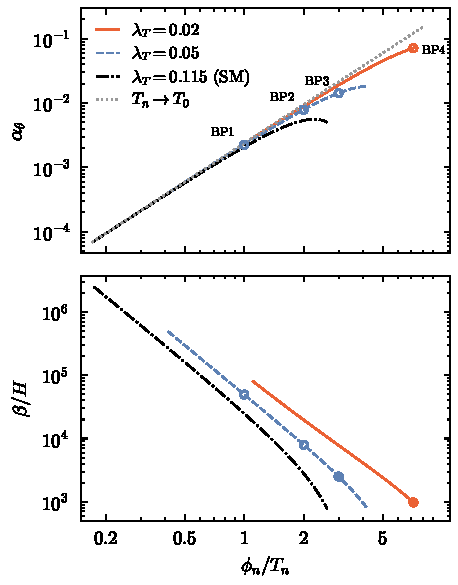
\includegraphics[width=0.5\linewidth]{../figs/strong_pt.pdf}
\caption{一般形の相転移の強さ $\alpha_\theta$（上）と速さ $\beta/H$（下）を、$\phi_n/T_n$ の関数として示す（手順 (2)）。$D$、$T_0$ は SM 的な値に固め、各 $\lambda_T$ で $E$ を SM 的な値から $0.995E_{\max}$ まで動かした。点線は $T_n\to T_0$ での上限 $(15D/\pi^2g_*)(\phi_n/T_n)^2$、丸は表~\ref{tab:bench} の基準点である。}
\label{fig:strong}
\end{figure}

\begin{table}[tbp]
\centering\small
\caption{手順 (3) のための基準点。BP1〜BP3 は $\lambda_T=0.05$ で $\phi_n/T_n=1$、$2$、$3$ となる点、BP4 は走査で最も強い点（$\lambda_T=0.02$、$E=0.995E_{\max}$）である。$D=0.166632$、$T_0=163.4953$~GeV、$g_*=106.75$ は共通である。}
\label{tab:bench}
\begin{tabular}{lllll}
\toprule
 & BP1 & BP2 & BP3 & BP4 \\
\midrule
$\lambda_T$ & $0.05$ & $0.05$ & $0.05$ & $0.02$ \\
$E$ & $0.022285$ & $0.042720$ & $0.062274$ & $0.054155$ \\
$R$ & $16.776$ & $4.5652$ & $2.1484$ & $1.1363$ \\
$T_c$ [GeV] & $168.597$ & $185.009$ & $223.623$ & $472.014$ \\
$T_n$ [GeV] & $167.794$ & $179.351$ & $199.960$ & $213.388$ \\
$\alpha(T_n)$ & $0.8485$ & $0.7715$ & $0.7121$ & $0.4693$ \\
$S_3/T$ & $148.68$ & $148.41$ & $147.97$ & $147.71$ \\
$\phi_n/T_n$ & $1$ & $2$ & $3$ & $7.163$ \\
$\alpha_\theta$ & $2.252\times10^{-3}$ & $7.886\times10^{-3}$ & $1.427\times10^{-2}$ & $7.145\times10^{-2}$ \\
$\alpha_e$ & $8.894\times10^{-3}$ & $2.906\times10^{-2}$ & $4.242\times10^{-2}$ & $1.160\times10^{-2}$ \\
$\beta/H$ & $4.958\times10^4$ & $7.926\times10^3$ & $2.496\times10^3$ & $9.742\times10^2$ \\
\bottomrule
\end{tabular}
\end{table}

\paragraph{手順 (3)：重力波と LISA の感度。}使った式は、すべて原論文で確かめた。$\kappa$ は Espinosa ら~\cite{espinosa10} の付録 A の式 (95)〜(102)、音波は Hindmarsh ら~\cite{hhrw17} の式 (23)、(35)、(36)、(43) と正誤表の式 (2)、衝撃波の補正は Caprini ら~\cite{caprini20} の式 (32)、乱流は Caprini ら~\cite{caprini16} の式 (16)〜(18)、(21)、LISA の感度は要求文書~\cite{scird} の式 (3) である。音波の振幅には、文献の間で食い違いがある。Caprini ら~\cite{caprini20} の式 (29) は、正誤表の $3$ の代わりに $1/c_s=\sqrt3$ を持ち、式 (32) の衝撃波の補正は $H_*R_*/\bar U_f$ の代わりに $H_*R_*/\sqrt K$ である。同じ $\tilde\Omega_{\mathrm{gw}}$ でそのまま使うと、本ノートの基準点では振幅がちょうど $1/2$ になる。Caprini ら~\cite{caprini16} の式 (13)〜(15) には衝撃波の補正がなく、ピークは $30$〜$190$ 倍大きい。本ノートでは、数値シミュレーションの原論文の正誤表による式~\eqref{eq:Osw} を使い、この差を振幅の不定性とみなす。

検算は五つ行った。(a) $\int C\,\dd\ln s=1.45539$ で、その逆数 $0.68710$ は式の $0.687$ と一致した。(b) $T_{\gamma,0}=2.725$~K から $\Omega_{\gamma,0}h^2=2.4711\times10^{-5}$ で、$F_{\mathrm{gw},0}(g_*=100)=3.5670\times10^{-5}$ は $3.57\times10^{-5}$ と相対 $9\times10^{-4}$ で一致した。(c) エントロピーの保存から求めた $H_{*,0}$ は、$T_*=100$~GeV、$g_*=100$ で $16.46\,\mu$Hz で、$16.5\,\mu$Hz と相対 $2\times10^{-3}$ で一致した。$f_p$ の係数 $(z_p/2\pi)H_{*,0}=26.20\,\mu$Hz は、$26\,\mu$Hz と $0.8\%$ で一致した。(d) $\kappa$ の近似式は、$v_w=c_s$ と Jouguet の速さ $v_J$ で、両側の値が相対 $10^{-6}$ 以内で一致し（$10^{-9}$ ずらした分の差）、$v_w=1$ で $\kappa_D$ になる。(e) PLS に接するべき乗のスペクトルの SNR は $10.000000$ である。LISA の $h^2\Omega_{\mathrm{sens}}$ の最小は $2.45$~mHz での $4.38\times10^{-12}$、PLS（SNR $=10$）の最小は $2.62$~mHz での $8.79\times10^{-14}$ である。

基準点の結果を表~\ref{tab:gw} と図~\ref{fig:gw} に示す。どの点でも $H_*\tau_{\mathrm{sh}}=0.009$〜$0.074$ と小さく、衝撃波ができて音波はハッブル時間の数 \% で終わる。乱流のピークは、$v_w=0.95$ のどの点でも音波のおよそ $1/550$ である。ただし、乱流は高い周波数で $f^{-5/3}$ とゆっくり下がるので、BP4 では $0.23$~Hz より上で音波を上回る。$v_w=0.95$ では、BP1〜BP4 のピークの周波数は $786$、$134$、$47$、$20$~mHz、ピークの $h^2\Omega_{\mathrm{gw}}$ は $3.2\times10^{-23}$〜$2.0\times10^{-15}$、SNR は $7.6\times10^{-15}$〜$0.014$ である。$v_w=0.44$ では $\kappa$ は大きくなるが、$R_*$ が $c_s$ で決まり、$f_p$ も高くなるので、SNR はさらに小さい。手順 (2) の走査の180点すべてで SNR を求めると、最大は BP4 の $0.014$ で、検出の目安の SNR $=10$ より3桁小さい。Caprini ら~\cite{caprini16} の大きい振幅を使っても、BP4 の SNR は $0.12$ である。

足りない理由は、$\beta/H$ が大きすぎ、強さも小さいことである。衝撃波で音波が早く終わると、$\Omega_{\mathrm{sw}}\propto K^{3/2}(H_*R_*)^2$ で、$H_*R_*\propto(\beta/H)^{-1}$ が効く。BP4 の $\alpha_\theta$ と $T_n$ のまま SNR $=10$ にするには $\beta/H\le134$ が要る（このとき $f_p=2.7$~mHz で、LISA の最も感度のよい周波数に来る）。BP4 の $\beta/H$ のままなら $\alpha_\theta\ge2.05$ が要る。一般形の走査では $\beta/H\ge7.5\times10^2$、$\alpha_\theta\le0.071$ なので、$D$ と $T_0$ を SM 的な値に固め、$\lambda_T\ge0.02$ とした範囲の一般形では、LISA で見える重力波は作れない。スクリプトは \texttt{gw\_spectrum.py} である。

\begin{figure}[tbp]
\centering
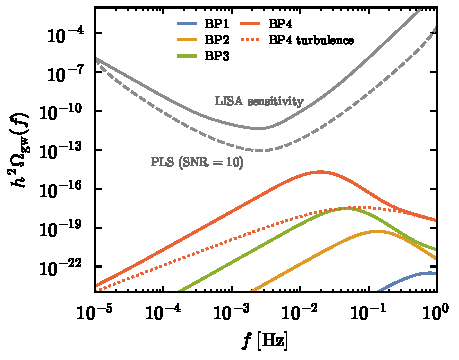
\includegraphics[width=0.5\linewidth]{../figs/gw_spectrum.pdf}
\caption{基準点の重力波のスペクトル（音波と乱流の和、$v_w=0.95$）と LISA の感度（手順 (3)）。灰色の実線は要求文書の感度 $h^2\Omega_{\mathrm{sens}}$、灰色の破線は SNR $=10$ の PLS、点線は BP4 の乱流の寄与である。}
\label{fig:gw}
\end{figure}

\begin{table}[tbp]
\centering\small
\caption{基準点の重力波（手順 (3)）。上は $v_w=0.95$、下は $v_w=0.44$ である。ピークは式~\eqref{eq:Osw}、\eqref{eq:Oturb} の $h^2\Omega$ の最大値、SNR は音波と乱流の和を式~\eqref{eq:snr} に入れた値である。}
\label{tab:gw}
\begin{tabular}{lllll}
\toprule
 & BP1 & BP2 & BP3 & BP4 \\
\midrule
\multicolumn{5}{l}{$v_w=0.95$} \\
$\kappa$ & $0.00348$ & $0.0120$ & $0.0216$ & $0.0988$ \\
$K$ & $7.83\times10^{-6}$ & $9.43\times10^{-5}$ & $3.03\times10^{-4}$ & $6.59\times10^{-3}$ \\
$H_*R_*$ & $5.61\times10^{-5}$ & $3.51\times10^{-4}$ & $1.11\times10^{-3}$ & $2.86\times10^{-3}$ \\
$H_*\tau_{\mathrm{sh}}$ & $0.0232$ & $0.0418$ & $0.0739$ & $0.0406$ \\
$f_p$ [mHz] & $786$ & $134$ & $47.1$ & $19.6$ \\
音波のピーク & $3.2\times10^{-23}$ & $5.2\times10^{-20}$ & $3.0\times10^{-18}$ & $2.0\times10^{-15}$ \\
乱流のピーク & $5.7\times10^{-26}$ & $9.4\times10^{-23}$ & $5.5\times10^{-21}$ & $3.6\times10^{-18}$ \\
SNR & $7.6\times10^{-15}$ & $2.3\times10^{-9}$ & $2.4\times10^{-6}$ & $1.4\times10^{-2}$ \\
\midrule
\multicolumn{5}{l}{$v_w=0.44$} \\
$\kappa$ & $0.00874$ & $0.0281$ & $0.0476$ & $0.174$ \\
$f_p$ [mHz] & $1293$ & $221$ & $77.6$ & $32.3$ \\
音波のピーク & $4.6\times10^{-23}$ & $6.8\times10^{-20}$ & $3.6\times10^{-18}$ & $1.7\times10^{-15}$ \\
SNR & $2.5\times10^{-15}$ & $7.0\times10^{-10}$ & $7.6\times10^{-7}$ & $3.7\times10^{-3}$ \\
\bottomrule
\end{tabular}
\end{table}

\FloatBarrier
\section{議論と今後}\label{sec:discussion}

\paragraph{今後。}第~\ref{sec:plan} 節の手順 (4) から順に進める。手順 (4) 以降の手計算（単一場の温度ポテンシャル）は、進めるにつれて付録に加える。

\appendix

\section{一般形と零温度の模型の対応、臨界温度の導出}\label{app:map}

\paragraph{係数の対応。}式~\eqref{eq:VT} を $V=\frac12m^2\phi^2+\frac g6\phi^3+\frac\lambda{24}\phi^4$ と比べると、$\frac12m^2=D(T^2-T_0^2)$、$\frac g6=-ET$、$\frac\lambda{24}=\frac{\lambda_T}4$ なので、$m^2=M^2=2D(T^2-T_0^2)$、$g=-6ET$、$\lambda=6\lambda_T$ である。よって $\alpha=3\lambda m^2/g^2=18\lambda_TM^2/(36E^2T^2)=\lambda_TM^2/(2E^2T^2)$ で、$M^2$ を入れると式~\eqref{eq:alphaT} を得る。逆に解くと $M^2=2\alpha E^2T^2/\lambda_T$ である。

\paragraph{極小と臨界温度。}零温度のノートの付録~G より、$f=g\phi/m^2$ について、二つ目の極小は $\alpha\le9/8$ で $f_-=-\frac{9}{2\alpha}\bigl(1+\sqrt{1-8\alpha/9}\bigr)$ にあり、$\alpha=1$ で $\phi=0$ と縮退する。$\phi=0$ は $m^2=M^2<0$、すなわち $\alpha<0$ で不安定になる。$\phi=(m^2/g)f=-M^2f/(6ET)$ である。$\alpha=9/8$ は $1-T_0^2/T^2=9/(8R)$ を与え、$T_1^2=T_0^2/(1-9E^2/(8\lambda_TD))$ である。このとき $f_-=-4$ で、$\phi_1=4M^2/(6ET)=\frac23\cdot\frac{2\cdot\frac98E^2T^2}{\lambda_T}\cdot\frac{1}{ET}=\frac{3ET}{2\lambda_T}$ である。$\alpha=1$ は $T_c^2=T_0^2/(1-E^2/(\lambda_TD))$ を与え、$f_-=-6$ から $\phi_c=M^2/(ET)=2ET_c/\lambda_T$ である。$\alpha\to0$ では $f_-\simeq-9/\alpha$ なので、$\phi_0=\frac{9M^2}{6\alpha ET}=\frac{3ET}{\lambda_T}$ である。

\paragraph{3次元の作用。}零温度のノートの $S_3=(m^3/g^2)S_3(\alpha)$ に $m=M$、$g^2=36E^2T^2$ を入れると $S_3/T=M^3S_3(\alpha)/(36E^2T^3)$ で、$M^3=(2\alpha/\lambda_T)^{3/2}E^3T^3$ から式~\eqref{eq:S3T} を得る。

\paragraph{SM 的な係数。}Dine らの式 (4)、(8)〜(11) は
\begin{equation*}
D=\frac{2m_W^2+m_Z^2+2m_t^2}{8v^2},\quad E=\frac{2m_W^3+m_Z^3}{4\pi v^3},\quad B=\frac{3(2m_W^4+m_Z^4-4m_t^4)}{64\pi^2v^4},\quad
T_0^2=\frac{m_h^2-8Bv^2}{4D}
\end{equation*}
と、$\lambda_T=\lambda-\frac{3}{16\pi^2v^4}\bigl[2m_W^4\ln\frac{m_W^2}{a_BT^2}+m_Z^4\ln\frac{m_Z^2}{a_BT^2}-4m_t^4\ln\frac{m_t^2}{a_FT^2}\bigr]$（$\ln a_B=2\ln4\pi-2\gamma_E$、$\ln a_F=2\ln\pi-2\gamma_E$、$\lambda=m_h^2/(2v^2)$）である。$T_c$ は、$\lambda_T(T_c)$ を使った式~\eqref{eq:crit} を反復で解いて求めた。

\section{核生成の条件と相転移の速さの導出}\label{app:nucl}

\paragraph{核生成の条件。}$\Gamma=T^4(S_3/(2\pi T))^{3/2}e^{-S_3/T}$ と $H=1.66\sqrt{g_*}T^2/M_{\mathrm{Pl}}$ を $\Gamma=H^4$ に入れて対数をとると、$4\ln T+\frac32\ln\frac{S_3}{2\pi T}-\frac{S_3}{T}=4\ln H$、すなわち式~\eqref{eq:nucl} を得る。$T=163.9$~GeV では $M_{\mathrm{Pl}}/(1.66\sqrt{g_*}T)=4.34\times10^{15}$ で、右辺は $144.0$ である。$S_3/T=148.8$ では左辺の対数の項が $4.7$ なので、両辺が釣り合う。$T_n$ は、$\ln(\Gamma/H^4)$ を $T$ の関数として Brent 法で解いて求めた。$\phi_n$ は $T_n$ での $f_-$ から $\phi=-M^2f_-/(6ET)$ で求めた。

\paragraph{相転移の速さ。}$S_3/T=(E/36)(2/\lambda_T)^{3/2}\alpha^{3/2}S_3(\alpha)$ を $\alpha$ で微分すると $\frac{\dd}{\dd\alpha}\frac{S_3}{T}=\frac{S_3}{T}\bigl[\frac3{2\alpha}+\frac{W}{S_3(\alpha)}\bigr]$ である（$\lambda_T$ は一定とする）。式~\eqref{eq:alphaT} から $T\frac{\dd\alpha}{\dd T}=2R\frac{T_0^2}{T^2}=2(R-\alpha)$ なので、式~\eqref{eq:betaH} を得る。数値の確かめでは、$S_3/T$ の中心差分を刻み $h=10^{-6}T_n$ と $h/2$ で求めて Richardson 外挿した。

\section{相転移の強さの導出}\label{app:strength}

\paragraph{熱力学の量。}各相の圧力は自由エネルギー密度の符号を変えたもので、前提 6 より $p_\pm=p_{\mathrm{rad}}-V_\pm$ である。ここで $p_{\mathrm{rad}}=\pi^2g_*T^4/90$、$V_+=V(0,T)=0$、$V_-=V(\phi_-(T),T)$ である。$e=T\,\dd p/\dd T-p$、$w=e+p=T\,\dd p/\dd T$ から
\begin{equation*}
e_\pm=\rho_{\mathrm{rad}}+V_\pm-T\frac{\dd V_\pm}{\dd T},\qquad
\theta_\pm=\frac{e_\pm-3p_\pm}{4}=V_\pm-\frac T4\frac{\dd V_\pm}{\dd T},\qquad
w_+=\frac43\rho_{\mathrm{rad}}
\end{equation*}
である。放射の部分は $e=3p$ なので $\theta$ に寄与しない。$\dd V_-/\dd T$ は $\phi_-$ の温度変化も含む全微分だが、$\partial V/\partial\phi=0$ が $\phi_-$ で成り立つので、$\dd V_-/\dd T=\partial V/\partial T|_{\phi=\phi_-}$ である。差を対称相から破れた相を引いたものとすると、$\Delta V=-V_-$、$\Delta\theta=-\theta_-=\Delta V-\frac T4\frac{\dd\Delta V}{\dd T}$、$\Delta e=-(e_--e_+)=\Delta V-T\frac{\dd\Delta V}{\dd T}$ である。Caprini らの式 (12)、(13) は $\alpha_\theta=4\Delta\theta/(3w_+)=\Delta\theta/\rho_{\mathrm{rad}}$、$\alpha_e=\Delta e/\rho_{\mathrm{rad}}$ になる。bag 模型（$V_+-V_-=\epsilon$ が温度によらない）では $\Delta\theta=\Delta e=\epsilon$ で、式 (9) の $\alpha$ に戻る。

\paragraph{極小での値。}$M^2=2D(T^2-T_0^2)$ と書くと、$V=\frac12M^2\phi^2-ET\phi^3+\frac{\lambda_T}4\phi^4$ で、極小の条件 $\phi^{-1}\partial V/\partial\phi=M^2-3ET\phi+\lambda_T\phi^2=0$ から $\frac{\lambda_T}4\phi_-^4=-\frac14M^2\phi_-^2+\frac34ET\phi_-^3$ である。これを入れると
\begin{equation*}
V_-=\frac14M^2\phi_-^2-\frac14ET\phi_-^3,\qquad
\frac T4\frac{\partial V}{\partial T}\Big|_{\phi_-}=\frac T4\bigl(2DT\phi_-^2-E\phi_-^3\bigr)=\frac12DT^2\phi_-^2-\frac14ET\phi_-^3
\end{equation*}
で、$\theta_-=\frac12D(T^2-T_0^2)\phi_-^2-\frac12DT^2\phi_-^2=-\frac12DT_0^2\phi_-^2$ を得る。よって $\Delta\theta=\frac12DT_0^2\phi_-^2$ で、$\rho_{\mathrm{rad}}=\pi^2g_*T^4/30$ で割ると式~\eqref{eq:alphatheta} になる。$\Delta V=-V_-=\frac{\phi_-^2}4(ET\phi_--M^2)$ も同時に得られる。$e_--\rho_{\mathrm{rad}}=V_--T\,\partial V/\partial T|_{\phi_-}=4\theta_--3V_-$、$e_+=\rho_{\mathrm{rad}}$ なので、$\Delta e=4\Delta\theta-3\Delta V$ で、式~\eqref{eq:alphae} を得る。

\paragraph{トレースが $T_0$ だけから来る理由。}$T_0=0$ なら $V(\phi,T)=T^4U(\phi/T)$ の形で、$V_-=T^4U(u_-)$（$u_-$ は $U$ の極小で、温度によらない）なので、$\theta_-=V_--\frac T4\cdot4V_-=0$ である。$\theta_-$ は $T$ について4次でない項、すなわち $-DT_0^2\phi^2$ だけから生じる。

\paragraph{$\alpha$ を通した別の導き方。}零温度のノートの変数で書くと、$\phi=(m^2/g)f$、$m^6/g^2=(2\alpha^3/9)E^4T^4/\lambda_T^3$ から $\Delta V=(E^4T^4/\lambda_T^3)h(\alpha)$、$h(\alpha)=-\frac{2\alpha^3}{9}v(f_-)$、$v(f)=\frac{f^2}2+\frac{f^3}6+\frac{\alpha f^4}{72}$ である。$T\,\dd\alpha/\dd T=2(R-\alpha)$ より $T\,\dd\Delta V/\dd T=4\Delta V+(E^4T^4/\lambda_T^3)h'(\alpha)\cdot2(R-\alpha)$ で、$\Delta\theta=-\frac{E^4T^4}{2\lambda_T^3}h'(\alpha)(R-\alpha)$ である。$v'(f_-)=0$ から $h'=-\frac29\bigl[3\alpha^2v(f_-)+\alpha^3f_-^4/72\bigr]$ で、極小の条件 $\alpha f_-^2/18=-f_-/2-1$ を使うと $v(f_-)=f_-^2(6+f_-)/24$、$\alpha f_-^4/72=-f_-^2(f_-+2)/8$ なので
\begin{equation*}
h'(\alpha)=-\frac29\cdot\frac{\alpha^2f_-^2}{8}\bigl[(6+f_-)-(f_-+2)\bigr]=-\frac{\alpha^2f_-^2}{9}=-\frac94\Bigl(1+\sqrt{1-\tfrac{8\alpha}9}\Bigr)^2
\end{equation*}
である。$\phi_-=-\alpha f_-ET/(3\lambda_T)$ より $-h'=(\lambda_T\phi_-/(ET))^2$ で、$R-\alpha=RT_0^2/T^2=\lambda_TDT_0^2/(E^2T^2)$ を入れると $\Delta\theta=\frac12DT_0^2\phi_-^2$ に戻る。

\paragraph{臨界温度での確かめ。}$T_c$（$\alpha=1$、$\phi_c=2ET_c/\lambda_T$、$M^2=2E^2T_c^2/\lambda_T$）では $ET_c\phi_c=M^2$ なので $\Delta V=0$ で、$\Delta e=4\Delta\theta=2DT_0^2\phi_c^2$ は潜熱 $L$ である。一方、潜熱を直接求めると、$L=-T_c\,\dd\Delta V/\dd T=T_c\,\partial V/\partial T|_{\phi_c}=T_c(2DT_c\phi_c^2-E\phi_c^3)=2\phi_c^2T_c^2(D-E^2/\lambda_T)$ である。$T_0^2=T_c^2(1-E^2/(\lambda_TD))$ より両者は等しい。

\paragraph{数値の確かめ。}$\Delta V$ は、$\phi_-$ の閉じた式の $0.5$〜$1.5$ 倍の区間で、$V(\phi,T)$ の極小を有界な Brent 法で求めた。$\dd\Delta V/\dd T$ は、刻み $h=10^{-5}(T_n-T_0)$ と $h/2$ の中心差分を Richardson 外挿して求めた。

\section{重力波の換算の導出}\label{app:gw}

\paragraph{流体の運動エネルギー。}Caprini ら~\cite{caprini20} の式 (10)、(11) では、泡1つのまわりの流体の運動エネルギーを、放出されたエネルギーで割ったものを効率 $\kappa$ とし、全エネルギーに対する割合を $K=\kappa\alpha/(1+\alpha)$ とする。Espinosa ら~\cite{espinosa10} の近似式は bag 模型の強さで書かれているが、Caprini らに従い $\alpha=\alpha_\theta$ を入れる。式 (22) の $K=\Gamma\bar U_f^2$ で、相対論的な流体の断熱指数 $\Gamma=w/e=4/3$ を使うと $\bar U_f=(3K/4)^{1/2}$ である。衝撃波ができるまでの時間は、流れの長さ $R_*$ を速さ $\bar U_f$ で割った $\tau_{\mathrm{sh}}=R_*/\bar U_f$ である（Caprini らの表 1、Hindmarsh らの式 (22)）。

\paragraph{泡の平均間隔。}核生成率が $\Gamma(t)=\Gamma_\star e^{\beta(t-t_\star)}$ で増え、泡が速さ $v_w$ で広がるとする（宇宙膨張は無視する）。時刻 $t$ に偽の真空が残る割合は $e^{-I(t)}$ で、$I(t)=\int_{-\infty}^t\dd t'\,\Gamma(t')\,\frac{4\pi}3v_w^3(t-t')^3$ である。$x=t-t'$ とおくと $I=\frac{4\pi}3v_w^3\Gamma(t)\int_0^\infty x^3e^{-\beta x}\dd x=\frac{8\pi v_w^3}{\beta^4}\Gamma(t)$ である。泡の数密度は、偽の真空で生まれる泡を数えて $n_b=\int\dd t\,\Gamma(t)e^{-I(t)}$ である。$u=I(t)$ とおくと $\dd u=\beta u\,\dd t$、$\Gamma=\beta^4u/(8\pi v_w^3)$ なので、$n_b=\frac{\beta^3}{8\pi v_w^3}\int_0^\infty e^{-u}\dd u=\frac{\beta^3}{8\pi v_w^3}$ である。平均間隔は $R_*=n_b^{-1/3}=(8\pi)^{1/3}v_w/\beta$ である。デフラグレーションでは、壁の前の衝撃波が音速で先に広がるので、$v_w$ を $c_s$ に置き換える（Caprini らの式 (6)）。$\beta=\dd\ln\Gamma/\dd t$ は、$\dd T/\dd t=-HT$ から $\beta=H\,T\,\dd(S_3/T)/\dd T$ で、式~\eqref{eq:betaH} の $\beta/H$ に $H_*$ を掛けたものである。

\paragraph{今日までの薄まり。}重力波は放射と同じく $a^{-4}$ で薄まるので、$\Omega_{\mathrm{gw},0}=\Omega_{\mathrm{gw},*}\,\rho_*a_*^4/(\rho_{c,0}a_0^4)$ である。$\rho_*=\frac{\pi^2}{30}g_*T_*^4$ で、エントロピーの保存 $g_sT^3a^3=$ 一定から $a_*/a_0=(g_{s0}/g_{s*})^{1/3}T_{\gamma,0}/T_*$ である（$T_{\gamma,0}$ は今日の CMB の温度）。よって
\begin{equation*}
F_{\mathrm{gw},0}=\frac{\pi^2}{30}g_*T_{\gamma,0}^4\Bigl(\frac{g_{s0}}{g_{s*}}\Bigr)^{4/3}\frac1{\rho_{c,0}}=\Omega_{\gamma,0}\Bigl(\frac{g_{s0}}{g_{s*}}\Bigr)^{4/3}\frac{g_*}{2},\qquad
\Omega_{\gamma,0}=\frac{\pi^2}{15}\frac{T_{\gamma,0}^4}{\rho_{c,0}}
\end{equation*}
である。$g_{s*}=g_*$ とすると、$g_*$ への依存は $g_*\cdot g_*^{-4/3}=g_*^{-1/3}$ である。$T_{\gamma,0}=2.725$~K、$\rho_{c,0}=3H_0^2M_{\mathrm{Pl}}^2/(8\pi)$ から $\Omega_{\gamma,0}h^2=2.4711\times10^{-5}$ で、$h=0.678$、$g_{s0}=3.91$、$g_*=100$ で $F_{\mathrm{gw},0}=3.567\times10^{-5}$ である。

\paragraph{周波数の換算。}周波数は $a^{-1}$ で下がる。$H_*$ を今日の周波数に直すと
\begin{equation*}
H_{*,0}=H_*\frac{a_*}{a_0}=1.66\sqrt{g_*}\,\frac{T_*^2}{M_{\mathrm{Pl}}}\Bigl(\frac{g_{s0}}{g_{s*}}\Bigr)^{1/3}\frac{T_{\gamma,0}}{T_*}
\end{equation*}
で、$T_*=100$~GeV、$g_*=100$ では $16.46\,\mu$Hz である（GeV から Hz へは $\hbar$ で直す）。$H_{*,0}$ は $T_*$ と $g_*^{1/2-1/3}=g_*^{1/6}$ に比例する。音波のスペクトルは $kR_*=z_p$ でピークを持つ（Hindmarsh らの VI 節）。$k$ は角波数なので、生じたときの周波数は $z_p/(2\pi R_*)$ で、今日は $f_p=\frac{z_p}{2\pi}\frac{H_{*,0}}{H_*R_*}$ である。$z_p=10$ で係数は $26.2\,\mu$Hz になり、Hindmarsh らの式 (43) の $26\,\mu$Hz にあたる。

\paragraph{感度と SNR。}特性歪み $h_c$ を $\langle h_{ij}h_{ij}\rangle=2\int h_c^2\,\dd\ln f$ で定め、感度曲線の規約 $h_c^2=fS_h$ をとる。このとき $\langle\dot h_{ij}\dot h_{ij}\rangle=2\int\dd f\,(2\pi f)^2S_h$ で、$\rho_{\mathrm{gw}}=\langle\dot h_{ij}\dot h_{ij}\rangle/(32\pi G)$ から $\dd\rho_{\mathrm{gw}}/\dd\ln f=\pi f^3S_h/(4G)$ である。$\rho_{c,0}=3H_0^2/(8\pi G)$ で割ると $\Omega=2\pi^2f^3S_h/(3H_0^2)$ で、両辺に $h^2$ を掛けると式~\eqref{eq:snr} の左の式になる。Caprini らの式 (34) は、この規約で要求文書の $S_h$ を使っている。SNR は Caprini らの式 (33) で、$T_{\mathrm{obs}}$ は観測期間に稼働率を掛けたものである。積分は $10^{-5}$〜$1$~Hz で、対数で等間隔な6001点の台形公式で行った。

\paragraph{べき乗のスペクトルに対する感度。}SNR は振幅に比例するので、$\Omega_\beta(f/f_{\mathrm{ref}})^\beta$ の SNR を $\rho_{\mathrm{th}}$ にする振幅は
\begin{equation*}
\Omega_\beta=\rho_{\mathrm{th}}\Bigl[T_{\mathrm{obs}}\int\dd f\,\frac{(f/f_{\mathrm{ref}})^{2\beta}}{\Omega_{\mathrm{sens}}(f)^2}\Bigr]^{-1/2}
\end{equation*}
である。PLS はその包絡線 $\Omega_{\mathrm{PLS}}(f)=\max_\beta\Omega_\beta(f/f_{\mathrm{ref}})^\beta$ である（Thrane と Romano の式 (29)、(30) で、SNR を式~\eqref{eq:snr} に替えたもの）。PLS に接するべき乗のスペクトルは、ちょうど SNR $=\rho_{\mathrm{th}}$ を持つ。$\rho_{\mathrm{th}}=10$、$f_{\mathrm{ref}}=1$~mHz とし、$\beta$ は $-8$〜$8$ を $0.05$ 刻みでとった。

\begin{thebibliography}{9}
\small
\bibitem{phi34note} $\phi^3+\phi^4$ 理論：1ループの構造、ユニタリー性、偽の真空の崩壊（$d=4$）（本リポジトリ \nolinkurl{models/phi34/ResearchNote/note.pdf}）。真空の構造（付録~G）、bounce の作用 $S_3(\alpha)$ と Dine らとの照合（手順 (9)、付録~L）。
\bibitem{dine92} M. Dine, R. G. Leigh, P. Y. Huet, A. D. Linde, D. A. Linde, ``Towards the theory of the electroweak phase transition,'' Phys. Rev. D \textbf{46}, 550 (1992), hep-ph/9203203。高温展開の一般形（式 (4)、(7)〜(11)）、臨界温度（式 (12)〜(16)）、$S_3/T$ の近似式（式 (26)、(27)）。
\bibitem{linde83} A. D. Linde, ``Decay of the false vacuum at finite temperature,'' Nucl. Phys. B \textbf{216}, 421 (1983); Erratum Nucl. Phys. B \textbf{223}, 544 (1983)。有限温度の崩壊率 $\Gamma\sim T^4e^{-S_3/T}$。
\bibitem{kajantie96} K. Kajantie, M. Laine, K. Rummukainen, M. E. Shaposhnikov, ``Is there a hot electroweak phase transition at $m_H\gtrsim m_W$?,'' Phys. Rev. Lett. \textbf{77}, 2887 (1996), hep-ph/9605288。格子計算による電弱相転移の終点。
\bibitem{caprini20} C. Caprini \textit{et al.}, ``Detecting gravitational waves from cosmological phase transitions with LISA: an update,'' JCAP \textbf{03} (2020) 024, arXiv:1910.13125。相転移の強さの定義（bag 模型の式 (8)〜(11)、トレースによる $\alpha_\theta$ の式 (12)、エネルギーの差による $\alpha_e$ の式 (13)）。音波の式 (29)〜(32)、SNR と感度の式 (33)、(34)、泡の平均間隔の式 (6)。
\bibitem{espinosa10} J. R. Espinosa, T. Konstandin, J. M. No, G. Servant, ``Energy budget of cosmological first-order phase transitions,'' JCAP \textbf{06} (2010) 028, arXiv:1004.4187。流体の運動への効率 $\kappa$ の近似式（付録 A の式 (95)〜(102)）。
\bibitem{hhrw17} M. Hindmarsh, S. J. Huber, K. Rummukainen, D. J. Weir, ``Shape of the acoustic gravitational wave power spectrum from a first order phase transition,'' Phys. Rev. D \textbf{96}, 103520 (2017); Erratum Phys. Rev. D \textbf{101}, 089902 (2020), arXiv:1704.05871。音波の全体の量（式 (23)）、スペクトルの形（式 (35)、(36)）、ピークの周波数（式 (43)）、正誤表の式 (2) と $\tilde\Omega_{\mathrm{gw}}=1.2\times10^{-2}$。
\bibitem{caprini16} C. Caprini \textit{et al.}, ``Science with the space-based interferometer eLISA. II: Gravitational waves from cosmological phase transitions,'' JCAP \textbf{04} (2016) 001, arXiv:1512.06239。乱流の式（式 (16)〜(18)、(21)）、音波の旧い式（式 (13)〜(15)）、SNR $=10$ の目安。
\bibitem{cds09} C. Caprini, R. Durrer, G. Servant, ``The stochastic gravitational wave background from turbulence and magnetic fields generated by a first-order phase transition,'' JCAP \textbf{12} (2009) 024, arXiv:0909.0622。乱流による重力波の解析的な計算。
\bibitem{thrane13} E. Thrane, J. D. Romano, ``Sensitivity curves for searches for gravitational-wave backgrounds,'' Phys. Rev. D \textbf{88}, 124032 (2013), arXiv:1310.5300。べき乗のスペクトルに対する感度（式 (29)、(30)）。
\bibitem{scird} LISA Science Study Team, ``LISA Science Requirements Document,'' ESA-L3-EST-SCI-RS-001, Issue 1.0 (2018)。歪みの感度（式 (3)）、観測期間と稼働率（3.6 節）。
\end{thebibliography}

\end{document}
